\chapter{Conjoncture et économie politique}
\section{Les faits empiriques}
Constat : l'état a plus de dépenses que de recettes  (déficit public) $\implies$ l'offre est constante et la demande $\nearrow \implies$ prix $\nearrow$ \newline

Par empirisme, le \textbf{traité de Maastricht (1992)} impose
\begin{center}
    \begin{itemize}
        \item Un déficit public $<$ 3 \% du PIB
        \item Une dette publique $<$ 60 \% du PIB
    \end{itemize}
\end{center}
\newpage
\section{Le modèle IS-LM} 
\begin{center}
    \textbf{IS : Investment Starving, LM : Loan Money}
\end{center}
\subsection{Modèle IS - Marché des biens et services}
Equilibre emploi-source macro-économique : 
\begin{center}
    \Large{\fbox{$
    Y = C + I + G
    $}}
\end{center}
Avec :
\begin{itemize}
    \item $Y$ : La production
    \item $C$ : la consommation des ménages
    \item $I$ : l'investissement privé
    \item $G$ : les dépenses de l'état
\end{itemize}
Equation de comportement de la consommation : 
\begin{center}
    \Large{\fbox{$
    C = c(Y - T) + C_{0}
    $}}
\end{center}
\begin{itemize}
    \item $c$ : la propension (tendance) à consommer : $c \in ]0;1[$
\end{itemize}
\begin{center}
    \Large{\fbox{$
    I = aY - br
    $}}
\end{center}
\begin{itemize}
    \item $r$  : le taux d'intérêt
\end{itemize}
 On a alors : 
\begin{center}
    \Large{\fbox{$
    Y = \frac{C_{0} + I + G - cT}{1 - c}
    $}}
\end{center}
Donc : 
\Large{$K = \frac{dY}{dG} = \frac{1}{1-c}$}, $K$ supérieur à 1 
: effet multiplicateur des dépenses publiques
\newpage
\subsection{Modèle LM - Marché de la monnaie}
\begin{center}
    \Large{\fbox{$
    \frac{M_{d}}{p} = eY - fr
    $}}
\end{center}
Avec : 
\begin{itemize}
    \item $e$ : constante strictement positive
    \item $f$ : constante strictement positive
    \item $M$ : quantité de monnaire de la part des agents
    \item $M_{s}$ : quantité de monnaie fournie par la banque centrale \footnote{La banque centrale produisant une quantité de monnaie exogène (qui ne dépend pas du système étudié) : $M_{s} = M = M_{d}$} 
    \item $M_{d}$ : demande de monnaie de la part des agents 
    \begin{itemize}
        \item Positivement du niveau de la demande : \textbf{motif de transactions}
        \item Négativement du taux d'intérêt : \textbf{motif de spéculation}
    \end{itemize}
\end{itemize}
\begin{center}
    \Large{\fbox{$
    M_{s} = M = M_{d}
    $}}
\end{center}
\newpage
\begin{center}
    \begin{figure}[hbt!]
        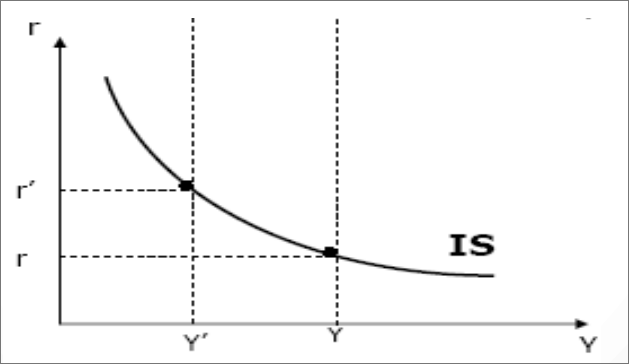
\includegraphics[scale=0.55]{Pics/Courbe_IS.png}
        \caption{Courbe IS - les couples $(Y,r)$ permettent l'équilibre du marché des biens et services}
    \end{figure}
    \begin{figure}[hbt!]
        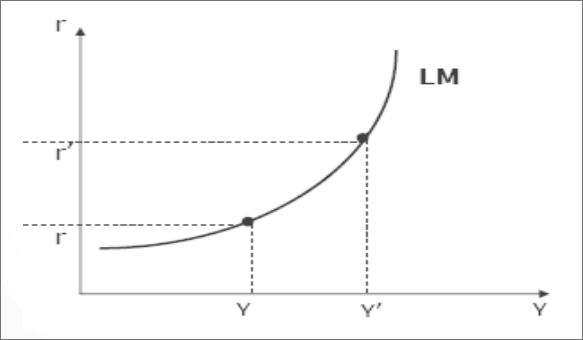
\includegraphics[scale=0.6]{Pics/Courbe_LM.png}
        \caption{Courbe LM - Les couples $(Y,r)$ permettent l'équilibre du marché de la monnaie} 
    \end{figure}    
\end{center}
\newpage
\subsection{Equilibre IS - LM}
\begin{figure}[hbt!]
    \centering
    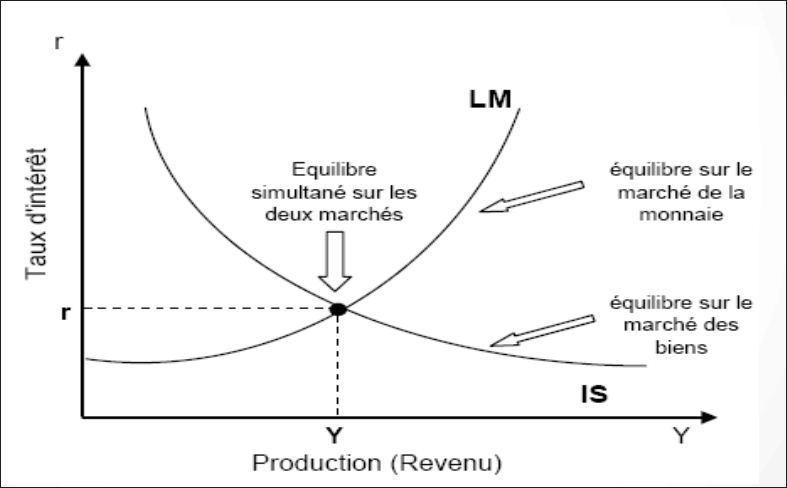
\includegraphics[scale=0.3]{Pics/Eq_IS_IM.png}
    \caption{Equilibre parfait}
\end{figure}

\begin{figure}[hbt!]
    \centering
    \begin{tabular}{cc}
      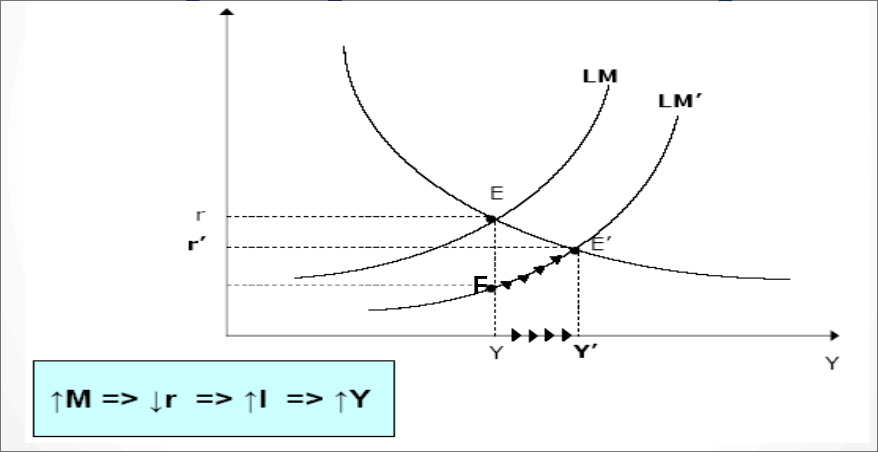
\includegraphics[scale=0.2]{Pics/Politque_expansioniste.png} &
      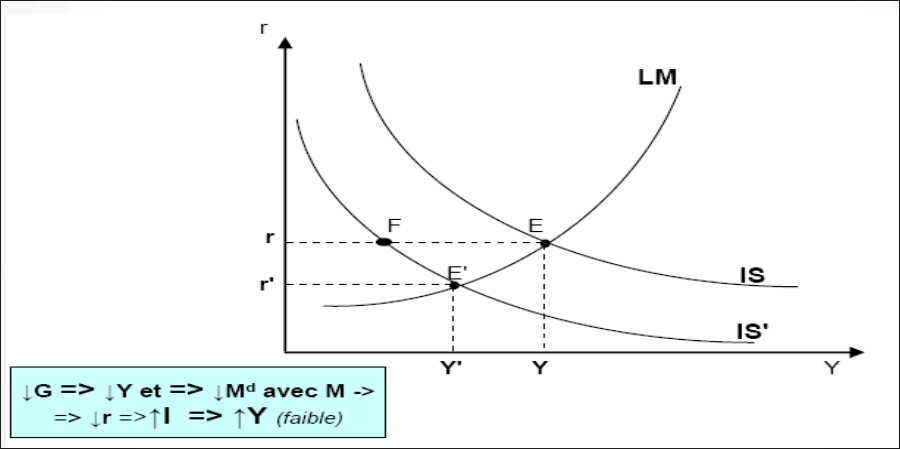
\includegraphics[scale=0.2]{Pics/Politique_budjetaire_restrictive.png} \\
      (a) & (b)\\
    \end{tabular}
    \caption{politique expansionniste (a) et politique de budjet restrictif (b)}
\end{figure}

\newpage
\section{La critique de la courbe de Philips}
\subsection{Principe d ela courbe de Philips}
\textbf{Relation négative entre le taux de chômage et le taux de croissance des salaires nominaux}. Relation utilisée pour démontrer la relation entre inflation et chômage et intégrer l'effet de la hausse des prix dans les modèles de prévision Keynésiens.
\begin{figure}[hbt!]
    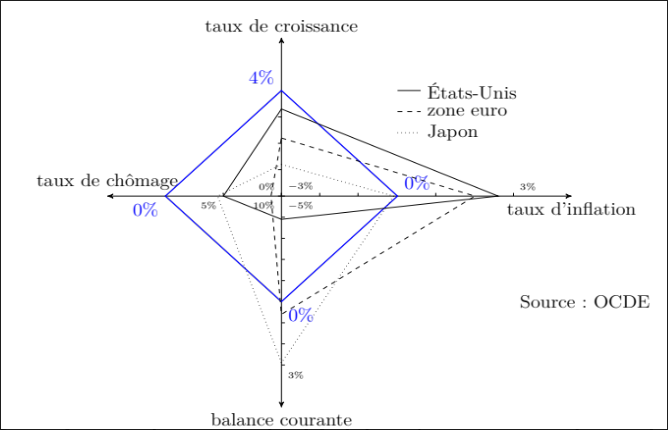
\includegraphics[scale=0.5]{Pics/Carre_magique.png}
    \caption{Carré magique de \textbf{Kaldor}}
\end{figure}
\newline
D'après le carré magique, il semble que plus il y a d'inflation, moins il y a de chômage : c'est la courbe de Philips.
\newpage
La courbe de Philips met en jeu 4 relations :
\begin{itemize}
    \item \textbf{Fonction d'offre} : \Large{\fbox{$
    P = (1 + t_{m})CM  = (1 + t_{m})(CFM + \frac{w}{PM}) 
    $}}
    \item \textbf{Relation inflation / salaire} : \Large{\fbox{$
    \frac{dP}{P} = \frac{dw}{w} - \frac{dPM}{PM}
    $}}
    \item \textbf{Relation salaire / chômage} : \Large{\fbox{$
    \overline{w} = \alpha(U - U_{n})
    $}}
    \item \textbf{Relation inflation / chômage} : \Large{\fbox{$
    \overline{P} = \alpha(U - U_{n}) - \overline{PM}
    $}}
\end{itemize}
Avec : 
\begin{itemize}
    \item $P$ : niveau général des prix
    \item $CM = CFM + CVM$ : coût moyen
    \item $t_{m}$ : taux de marge 
    \item $CVM = w\frac{L}{Y} = \frac{w}{PM}$ : coût variable moyen (salaire nominal) 
    \item $PM$ : produit moyen
    \item $U_{n}$ : taux de chômage naturel (plein emploi)
    \item $U$ : taux de chômage effectif \footnote{$
    U = U_{n}$ : marché du travail en équilibre : \textbf{NAWRU} (Non-Accelerating-Wage Rate of Unemployement
    $U sup U_{n}$ : concurrence entre les travailleurs $\implies$ baisse des salaires : plus de candidats que d'offres de poste
    \newline
    $U inf U_{n}$ : concurrence entre les employeurs $\implies$ salaires à la hausse : plus de postes à pourvoir que de candidats : notion de \textbf{NAIRU} (Non-Accelerating-Inflation Rate of Unemployement), le taux de chômage qui n'accelère pas l'inflation.
    En effet, si la hausse de salaires est plus importante que le taux de croissance de la productivité, l'inflation augmentera. Si le taux de chômage est inférieur au NAIRU, l'inflation augmentera.
     }
    \item $\alpha$ négatif
\end{itemize}
\newpage
\subsection{Solow-Samuelson}
On a : 
\begin{center}
    \Large{\fbox{$
    p =(1 + t_{m})w\frac{L}{Q}
    $}}
\end{center}
Alors on obtient : \footnote{On considère $t_{m}$ constant et en log différenciant}
\begin{center}
    \Large{\fbox{$
    \pi = g_{p} = g_{w} - \mu
    $}}
\end{center}
Avec : 
\begin{itemize}
    \item $\pi$ : taux d'inflation
    \item $g_{w}$ : taux de croissance des salaires
    \item $\mu = \frac{Q}{L}$ : taux de croissance de la productivité du travail
\end{itemize}
\begin{figure}[hbt!]
    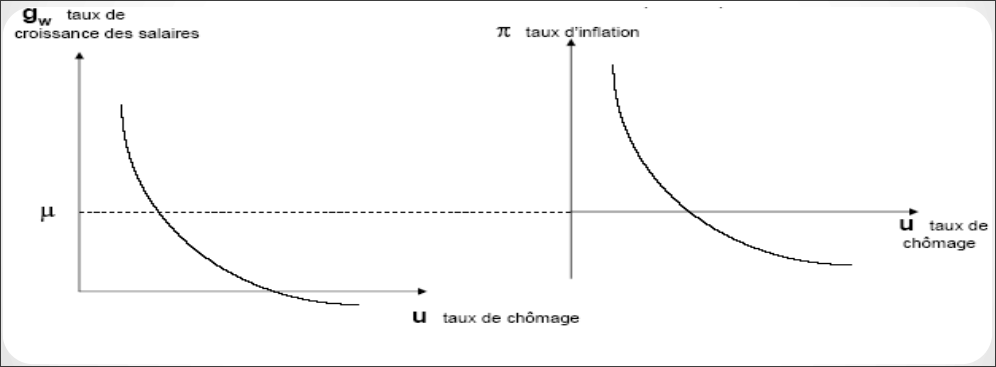
\includegraphics[scale = 0.4]{Pics/Solow_Samuelson.png}
\end{figure}
\newpage
\subsection{La critique de Friedman}
\begin{figure}[hbt!]
    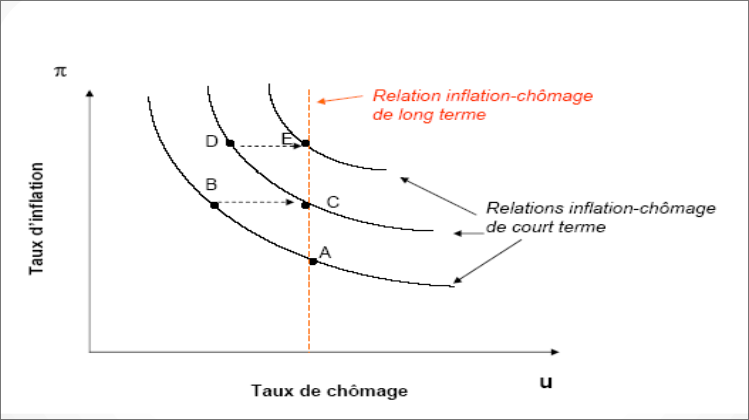
\includegraphics[scale = 0.4]{Pics/Critique_Friedman.png}
\end{figure}
Lors d'une relance budjétaire, les individus sont poussés à consommer plus car les salaires augmentent. Les individus consomment plus, la demande éclate et l'offre est à peu près constance $\implies$ les prix augmentent \footnote{Cf. théorie de l'offre et de la demande} : ils sont victimes d'une \textbf{illusion budjétaire}. Les relances budjétaires n'ont que pour conséquence l'inflation sur le long terme.
\subsection{Les anticipations rationnelles de Lucas}
Face à ces relances budjétaires, les individus réagissent en connaissance de cause. \textbf{Attention : le raisonnement rationnel se repose sur l'information disponible, l'anticipation peut être inexacte} 
\newpage
\begin{figure}[hbt!]
    \centering
    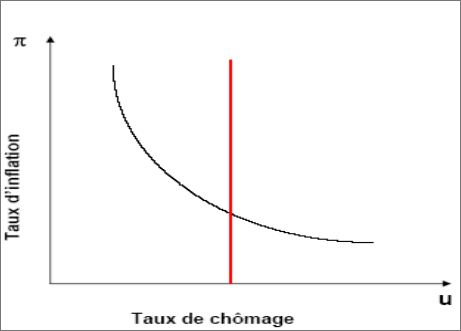
\includegraphics[scale=0.5]{Pics/anticipation_rationnelle_philips.png}
    \caption{Courbe de Philips \textcolor{BrickRed}{en rouge} avec une anticipation rationnelle, autant sur le court comme sur le long terme}
\end{figure}
\section{Le chômage}
\subsection{Définition}
Pour être au chômage, il faut réunir 3 conditions :
\begin{itemize}
    \item être sans emploi
    \item etre disponible pour occuper un emploi
    \item etre à la recherche d'un emploi
\end{itemize} 
Population \textbf{inactive} : \newline

Population qui n'as pas d'emploi et qui n'en cherche pas \newline

Population \textbf{active} : \newline
Population d'actifs occupés et de chômeurs
\newpage
\subsection{Autres Définitions}
Taux d'activité : 
\begin{center}
    \Large{\fbox{$
    a = \frac{PA}{PAA}
    $}}
\end{center}
Taux de chômage : 
\begin{center}
    \Large{\fbox{$
    u = \frac{U}{PAA}
    $}}
\end{center}
Taux d'emploi : 
\begin{center}
    \Large{\fbox{$
    e = \frac{Ne}{PAA}
    $}}
\end{center}
Avec : 
\begin{itemize}
    \item $Ne$ : nombre d'emploi
    \item $U$ : nombre de chômeurs
    \item $PAA$ : population en âge de travailler (15-64 ans)
    \item $PA$ : population active \newline
\end{itemize}
\textbf{Vulnérabilité} : rique de tomber au chômage. Ration entre la population au chômage depuis un an et la population active occupée.
\newline
\textbf{Employabilité} : Probabilité de sortir du chômage. Ratio entre le nombre de chômeurs ayant moins d'un an d'ancienneté et le nombre total de chômeurs.
\newpage
\subsection{Chômage structurel}
Le \textbf{chômage structurel} est un chômage \textbf{persistant}. Il s'explique par des causes \textbf{institutionnelles} comme le droit, la culture patronale et syndicale...
\newline

En France et comme dans beaucoup de pays en Europe, le chômage est persistant, structurel, - au contraire des Etats-Unis ou le chômage est plutôt d'origine conjoncturel - malgrès les politiques visant à réduire le chômage. Pourquoi autant de chômage ?
\begin{itemize}
    \item Insufisance de consommation \footnote{Cf. théorie Keynésienne}
    \item Rigidité des salaires à la baisse \footnote{Cf. théorie néoclassique}
    \item Les syndicats sont plus puissants
    \item La législation est restrictive sur le licenciement \footnote{On constat aujourd'hui plus de flexibilité sur les contrats de travail (séparation à l'amiable), les textes de loi sur le licenciement sont plus rigides que dans les faits et un retour à l'emploi plus sollicité}
    \item Les indémnisations chômages sont plus grandes
\end{itemize}
Solutions :
\begin{itemize}
    \item Baisser le coût du travail pour la catégorie sociale la plus touchée par le chômage : les ouvriers non qualifiés
    \item Inciter un retour au travail en faisant apparaître des écarts plus importants entre le salaire d'un travailleur et les indémnités chômage 
    \footnote{Des études empiriques montrent qu'il n'y a pas de réelles corrélations entre la quantité d'indemnités chômage et le temps passé au chômage, les seules mesures efficaces restent la mise en place d'aides pour la recherche au travail et des sanctions si l'individus recherche peu ou pas de travail. Les minimas sociaux sont eux aussi imparfaits car dès la reprise du travail, l'actif occupé perd ses allocations sociales qui compensaient le revenu minimum.}
\end{itemize}
\newpage
\subsection{Chômage conjoncturel}
\subsubsection{Loi d'Okun}
Lien entre les variations du taux de chômage et le taux de croissance pendant un cycle \newline

Les chômage conjoncturel : un chômage non persistant comme celui au Etats-Unis.